% Created by tikzDevice version 0.12.3 on 2020-04-18 17:47:30
% !TEX encoding = UTF-8 Unicode
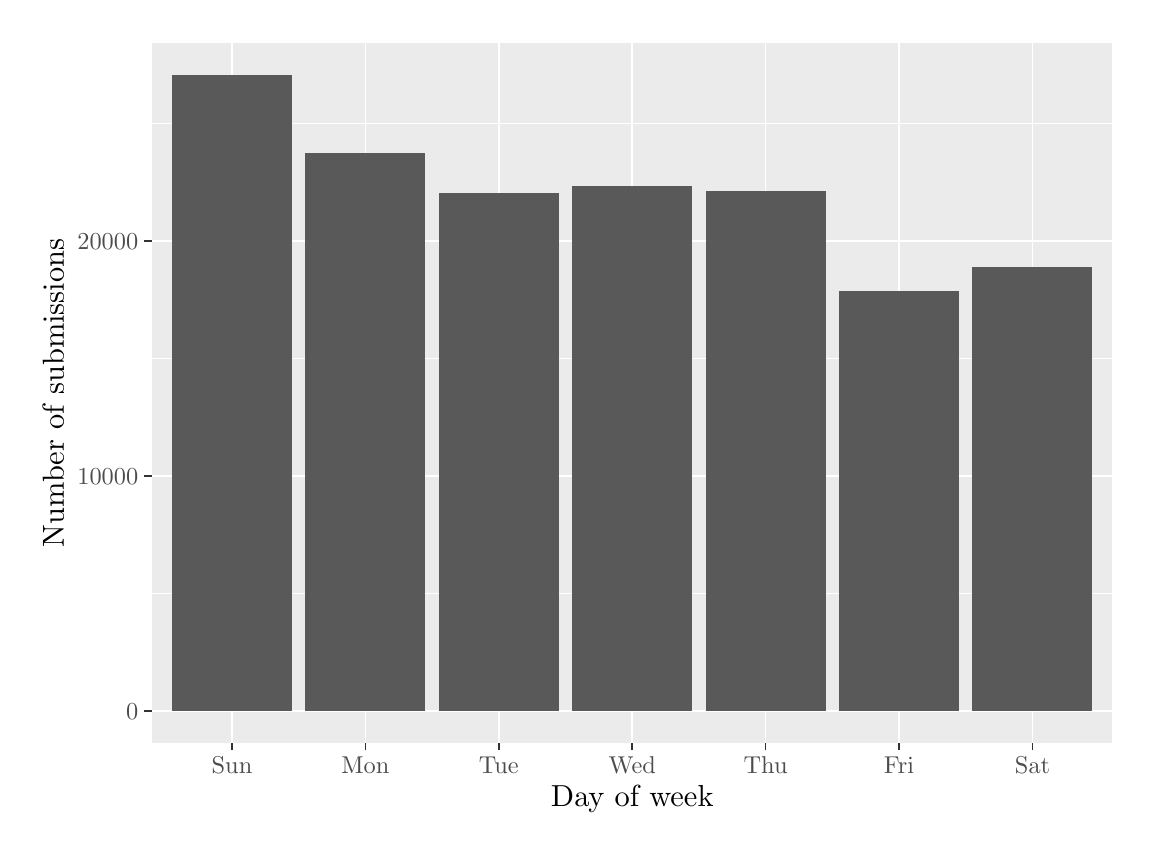
\begin{tikzpicture}[x=1pt,y=1pt]
\definecolor{fillColor}{RGB}{255,255,255}
\path[use as bounding box,fill=fillColor,fill opacity=0.00] (0,0) rectangle (397.48,289.08);
\begin{scope}
\path[clip] (  0.00,  0.00) rectangle (397.48,289.08);
\definecolor{drawColor}{RGB}{255,255,255}
\definecolor{fillColor}{RGB}{255,255,255}

\path[draw=drawColor,line width= 0.6pt,line join=round,line cap=round,fill=fillColor] (  0.00,  0.00) rectangle (397.48,289.08);
\end{scope}
\begin{scope}
\path[clip] ( 44.91, 30.69) rectangle (391.98,283.58);
\definecolor{fillColor}{gray}{0.92}

\path[fill=fillColor] ( 44.91, 30.69) rectangle (391.98,283.58);
\definecolor{drawColor}{RGB}{255,255,255}

\path[draw=drawColor,line width= 0.3pt,line join=round] ( 44.91, 84.63) --
	(391.98, 84.63);

\path[draw=drawColor,line width= 0.3pt,line join=round] ( 44.91,169.54) --
	(391.98,169.54);

\path[draw=drawColor,line width= 0.3pt,line join=round] ( 44.91,254.44) --
	(391.98,254.44);

\path[draw=drawColor,line width= 0.6pt,line join=round] ( 44.91, 42.18) --
	(391.98, 42.18);

\path[draw=drawColor,line width= 0.6pt,line join=round] ( 44.91,127.09) --
	(391.98,127.09);

\path[draw=drawColor,line width= 0.6pt,line join=round] ( 44.91,211.99) --
	(391.98,211.99);

\path[draw=drawColor,line width= 0.6pt,line join=round] ( 73.83, 30.69) --
	( 73.83,283.58);

\path[draw=drawColor,line width= 0.6pt,line join=round] (122.04, 30.69) --
	(122.04,283.58);

\path[draw=drawColor,line width= 0.6pt,line join=round] (170.24, 30.69) --
	(170.24,283.58);

\path[draw=drawColor,line width= 0.6pt,line join=round] (218.45, 30.69) --
	(218.45,283.58);

\path[draw=drawColor,line width= 0.6pt,line join=round] (266.65, 30.69) --
	(266.65,283.58);

\path[draw=drawColor,line width= 0.6pt,line join=round] (314.86, 30.69) --
	(314.86,283.58);

\path[draw=drawColor,line width= 0.6pt,line join=round] (363.06, 30.69) --
	(363.06,283.58);
\definecolor{fillColor}{gray}{0.35}

\path[fill=fillColor] ( 52.14, 42.18) rectangle ( 95.52,272.08);

\path[fill=fillColor] (100.34, 42.18) rectangle (143.73,243.83);

\path[fill=fillColor] (148.55, 42.18) rectangle (191.93,229.47);

\path[fill=fillColor] (196.75, 42.18) rectangle (240.14,231.81);

\path[fill=fillColor] (244.96, 42.18) rectangle (288.34,230.01);

\path[fill=fillColor] (293.16, 42.18) rectangle (336.55,193.93);

\path[fill=fillColor] (341.37, 42.18) rectangle (384.75,202.48);
\end{scope}
\begin{scope}
\path[clip] (  0.00,  0.00) rectangle (397.48,289.08);
\definecolor{drawColor}{gray}{0.30}

\node[text=drawColor,anchor=base east,inner sep=0pt, outer sep=0pt, scale=  0.88] at ( 39.96, 39.15) {0};

\node[text=drawColor,anchor=base east,inner sep=0pt, outer sep=0pt, scale=  0.88] at ( 39.96,124.05) {10000};

\node[text=drawColor,anchor=base east,inner sep=0pt, outer sep=0pt, scale=  0.88] at ( 39.96,208.96) {20000};
\end{scope}
\begin{scope}
\path[clip] (  0.00,  0.00) rectangle (397.48,289.08);
\definecolor{drawColor}{gray}{0.20}

\path[draw=drawColor,line width= 0.6pt,line join=round] ( 42.16, 42.18) --
	( 44.91, 42.18);

\path[draw=drawColor,line width= 0.6pt,line join=round] ( 42.16,127.09) --
	( 44.91,127.09);

\path[draw=drawColor,line width= 0.6pt,line join=round] ( 42.16,211.99) --
	( 44.91,211.99);
\end{scope}
\begin{scope}
\path[clip] (  0.00,  0.00) rectangle (397.48,289.08);
\definecolor{drawColor}{gray}{0.20}

\path[draw=drawColor,line width= 0.6pt,line join=round] ( 73.83, 27.94) --
	( 73.83, 30.69);

\path[draw=drawColor,line width= 0.6pt,line join=round] (122.04, 27.94) --
	(122.04, 30.69);

\path[draw=drawColor,line width= 0.6pt,line join=round] (170.24, 27.94) --
	(170.24, 30.69);

\path[draw=drawColor,line width= 0.6pt,line join=round] (218.45, 27.94) --
	(218.45, 30.69);

\path[draw=drawColor,line width= 0.6pt,line join=round] (266.65, 27.94) --
	(266.65, 30.69);

\path[draw=drawColor,line width= 0.6pt,line join=round] (314.86, 27.94) --
	(314.86, 30.69);

\path[draw=drawColor,line width= 0.6pt,line join=round] (363.06, 27.94) --
	(363.06, 30.69);
\end{scope}
\begin{scope}
\path[clip] (  0.00,  0.00) rectangle (397.48,289.08);
\definecolor{drawColor}{gray}{0.30}

\node[text=drawColor,anchor=base,inner sep=0pt, outer sep=0pt, scale=  0.88] at ( 73.83, 19.68) {Sun};

\node[text=drawColor,anchor=base,inner sep=0pt, outer sep=0pt, scale=  0.88] at (122.04, 19.68) {Mon};

\node[text=drawColor,anchor=base,inner sep=0pt, outer sep=0pt, scale=  0.88] at (170.24, 19.68) {Tue};

\node[text=drawColor,anchor=base,inner sep=0pt, outer sep=0pt, scale=  0.88] at (218.45, 19.68) {Wed};

\node[text=drawColor,anchor=base,inner sep=0pt, outer sep=0pt, scale=  0.88] at (266.65, 19.68) {Thu};

\node[text=drawColor,anchor=base,inner sep=0pt, outer sep=0pt, scale=  0.88] at (314.86, 19.68) {Fri};

\node[text=drawColor,anchor=base,inner sep=0pt, outer sep=0pt, scale=  0.88] at (363.06, 19.68) {Sat};
\end{scope}
\begin{scope}
\path[clip] (  0.00,  0.00) rectangle (397.48,289.08);
\definecolor{drawColor}{RGB}{0,0,0}

\node[text=drawColor,anchor=base,inner sep=0pt, outer sep=0pt, scale=  1.10] at (218.45,  7.64) {Day of week};
\end{scope}
\begin{scope}
\path[clip] (  0.00,  0.00) rectangle (397.48,289.08);
\definecolor{drawColor}{RGB}{0,0,0}

\node[text=drawColor,rotate= 90.00,anchor=base,inner sep=0pt, outer sep=0pt, scale=  1.10] at ( 13.08,157.13) {Number of submissions};
\end{scope}
\end{tikzpicture}
